%%%%%%%%%%%%%%%%%%%%%%%%%%%%%%%%%%%%%%%%%%%%%%%%%%%%%%%%%%%%
%%% LIVECOMS ARTICLE TEMPLATE FOR BEST PRACTICES GUIDE
%%% ADAPTED FROM ELIFE ARTICLE TEMPLATE (8/10/2017)
%%%%%%%%%%%%%%%%%%%%%%%%%%%%%%%%%%%%%%%%%%%%%%%%%%%%%%%%%%%%
%%% PREAMBLE
\documentclass[9pt,lessons]{livecoms}
% Use the 'onehalfspacing' option for 1.5 line spacing
% Use the 'doublespacing' option for 2.0 line spacing
% Use the 'lineno' option for adding line numbers.
% Use the 'pubversion' option for adding the citation and publication information to the document footer.
% The 'bestpractices' option for indicates that this is a best practices guide.
% Omit the bestpractices option to remove the marking as a LiveCoMS paper.
% Please note that these options may affect formatting.

\usepackage{lipsum} % Required to insert dummy text
\usepackage[version=4]{mhchem}
\usepackage{siunitx}
\DeclareSIUnit\Molar{M}
\usepackage[italic]{mathastext}
\usepackage{amsmath}
\graphicspath{{assets/}}
\DeclareGraphicsExtensions{.jpg,.png,.eps}
\usepackage{geometry}
\usepackage{pdflscape}
%%%%%%%%%%%%%%%%%%%%%%%%%%%%%%%%%%%%%%%%%%%%%%%%%%%%%%%%%%%%
%%% IMPORTANT USER CONFIGURATION
%%%%%%%%%%%%%%%%%%%%%%%%%%%%%%%%%%%%%%%%%%%%%%%%%%%%%%%%%%%%

\newcommand{\versionnumber}{1.0}  % you should update the minor version number in preprints and major version number of submissions.
\newcommand{\githubrepository}{\url{https://github.com/rodrigogalindo/DNA_salt_livecoms}} 

%%%%%%%%%%%%%%%%%%%%%%%%%%%%%%%%%%%%%%%%%%%%%%%%%%%%%%%%%%%%
%%% ARTICLE SETUP
%%%%%%%%%%%%%%%%%%%%%%%%%%%%%%%%%%%%%%%%%%%%%%%%%%%%%%%%%%%%
\title{Lessons learned in atomistic simulation of double-stranded DNA: Solvation and salt concerns. [Article v\versionnumber]}

\author[1]{Rodrigo Galindo-Murillo}
\author[1*]{Thomas E. Cheatham III}
\affil[1]{Department of Medicinal Chemistry, L. S. Skaggs Pharmacy Institute, University of Utah, Salt Lake City, UT 84112}

\corr{rodrigo.galindo@utah.edu}{RG-M}
\corr{tec3@utah.edu}{TEC3}

\blurb{This LiveCoMS document is maintained online on GitHub at \githubrepository; to provide feedback, suggestions, or help improve it, please visit the GitHub repository and participate via the issue tracker.}

%%%%%%%%%%%%%%%%%%%%%%%%%%%%%%%%%%%%%%%%%%%%%%%%%%%%%%%%%%%%
%%% PUBLICATION INFORMATION
%%% Fill out these parameters when available
%%% These are used when the "pubversion" option is invoked
%%%%%%%%%%%%%%%%%%%%%%%%%%%%%%%%%%%%%%%%%%%%%%%%%%%%%%%%%%%%
\pubDOI{10.XXXX/YYYYYYY}
\pubvolume{<volume>}
\pubyear{<year>}
\articlenum{<number>}
\datereceived{Day Month Year}
\dateaccepted{Day Month Year}

%%%%%%%%%%%%%%%%%%%%%%%%%%%%%%%%%%%%%%%%%%%%%%%%%%%%%%%%%%%%
%%% ARTICLE START
%%%%%%%%%%%%%%%%%%%%%%%%%%%%%%%%%%%%%%%%%%%%%%%%%%%%%%%%%%%%
\begin{document}

\begin{frontmatter}
\maketitle

\begin{abstract}
Nucleic acids are highly charged macromolecules sensitive to their
surroundings of water, salt, and other biomolecules. Molecular
dynamics simulations with accurate biomolecular force fields provide a
detailed atomistic view into DNA and RNA that has been useful to study
the structure and dynamics of these molecules and their biological
relevance. In this work we study the Drew-Dickerson dodecamer duplex
with the sequence d(GCGCAATTGCGC)$_{2}$ in three different
salt concentrations and using different monvalent salt types to detect
possible structural influence. Overall, the DNA shows no major
structural changes regardless of amount or type of monovalent ions used. Our
results show that only at very high salt conditions (5M) is a small
structural effect observed in the DNA duplex, which mainly consist of
narrowing of the grooves due to increased residence of ions. We
also present the importance of sampling time to achieve a converged
ensemble, which is of major relevance in any simulation to avoid
biased or non-meaningful results.
\end{abstract}

\end{frontmatter}


%%%%%%%%%%%%%%%%%%%%%%%%%%%%%%%%%%%%%%%%%%%%%%%%%%%%%%%%%%%%
%%% INTRODUCTION
%%%%%%%%%%%%%%%%%%%%%%%%%%%%%%%%%%%%%%%%%%%%%%%%%%%%%%%%%%%%
\section{Introduction}

\begin{figure*}[h]
\centering
\includegraphics[width=\linewidth]{1us-rms-ALL-inner-avg_ref-bsc0}
\caption{Left: normalized populations of RMSD values at three different concentrations considering only the 10 internal base pairs. Using the net-neutralizing (NaCl) simulation of the Dickerson dodecamer with a
  \SI{1}{\micro\second} duration, we calculated and extracted an average structure to use as a common reference for the RMSD calculations. Right: root mean square fluctuations per residue. Top to
  bottom is 200mM, 1M and 5M respectively.}
\label{1us-rms-ALL-inner-avg_ref-bsc0}
\end{figure*}

Monovalent and divalent cation interactions with nucleic acids play a
major role in their conformational structure, dynamics and
function\cite{Sharp1995}. The highly charged nature of nucleic acids
makes them highly sensitive to the ionic conditions in the
environment\cite{Saenger1988}. This environment is responsible for
several DNA structural rearrangements that have been experimentally
observed, changes that influence its biological function and binding to proteins
and other ligands\cite{McFail-Isom1999}. The most significant, and
arguably the most biologically relevant, DNA helical conformational
transition is the B$\rightarrow$A transition that is related to both
salt conditions and water activity\cite{Kulkarni2017,Waters2016}. In
low humidity – high salt conditions, interstrand phosphate repulsion
increases resulting the formation of A-form DNA, which is stabilized
by the presence of monovalent cations and phosphate bridging waters in
an economy of hydration\cite{Kulkarni2017,Saenger1986,Cheatham3rd1997}.

Other examples of conformational changes induces by monovalent ionic and solvent
environment include the conversion of B to Z-DNA in a GC-rich sequence
at high salt concentration\cite{Saenger1988}, stabilization of guanine
quadruplexes by a central Na$^{+}$ or K$^{+}$
ion\cite{Bhattacharyya2016} and formation of
the C-DNA fiber stabilized by lithium\cite{Langridge1960,Marvin1961}. RNA
biopolymers are also highly sensitive to ions and ionic
conditions. Folding, biological activity and functionality of RNA has
been found to be highly dependent on the type and concentration of
mono$-$ and divalent ions\cite{jenkins2017,bevil2016,westhof2000,
  westhof2001}.

Molecular dynamics simulations have provided extensive insight over
the last three decades about the interactions of mono-\cite{Cheatham3rd2013,feig,hamelberg1} and divalent
ions with nucleic acids\cite{Cheatham3rd2013,panteva1} including the
B$\rightarrow$A
transition\cite{Cheatham3rd1997,Cheatham3rd1996,mazurak,pastor,Kulkarni2017}. One of
our research directions over the last decade has been to utilize
molecular dynamics simulation methodologies to probe the influence of
ion concentration and identity on the structure and dynamics of
double-stranded DNA. An ambition was to spontaneously model the high
salt concentration B$\rightarrow$A helical transitions observed
experimentally and also to understand the impact of different
monovalent ions on DNA structure and dynamics.  Multiple monovalent
ion additive force field models have been developed\cite{mamatkulov,liwang,jeejoongyoo}, and these include
the Åqvist cation set\cite{Aqvist1990}, Dang ion set\cite{Smith1994},
Jensen—Jorgensen OPLS set\cite{Zichi1995}, Merz—Li\cite{Merzions}, and the
Joung—Cheatham ion parameters\cite{Joung2008,Joung2008a}.  Previously
published research has focused on the influence of salt types and salt
conditions on DNA structure and dynamics, however, most of this work
has involved very short simulations which are unlikely to be
converged. Orozco and co-workers investigated the influence of various
ion models on a small 6-mer DNA duplex using 500 mM of NaCl and KCl, in independent simulations, with 50
ns of unrestrained fully solvated MD. The results show a lack
of significant difference in the structural properties of the tested
DNA model, regardless of the ion model. Additionally, using
statistical methodologies to assess deviations between data sets, they
evaluated the DNA dynamics observed in the DNA trajectories,
concluding that the simulations are indistinguishable regardless of
the ion model used\cite{modesto09}. Also from the Orozco group, a
series of simulations of DNA were performed to study the Na$^{+}$
distribution and lifetime of the ions within the minor
groove\cite{Rueda2004}. They report no influence on the structure of
DNA due to the presence of 200mM of salt concentration using 10 ns of
sampling time. Yin and collaborators performed a series of simulations
at 0.46 M, 1.86 M and 3.27 M of NaCl salt concentration to study the
influence of salt concentration on the A$\rightarrow$B
transition\cite{Song2006}.  In each set of simulations the A-DNA
starting structures converted to B-DNA like structures within a
sampling time of 1.5 ns with no drastic influence within the B- like
conformation other than at high salt where the transition is slower.
Regarding the use of a polarizable force field to study the effects of
salt concentration in DNA, Savelyev and MacKerell report that the
inclusion of polarization effects does indeed produce differences in
solution scattering profiles when compared with both CHARMM 36 and
AMBER bsc0 force fields\cite{Rueda2004}. Their work includes both $\sim$100
mM of NaCl and independently $\sim$100 mM NaCl with the addition of $\sim$50 mM Tris$\cdot$HCl
aqueous buffer to compare directly to experimental X-ray scattering
data. From their simulations, they calculate the solution scattering
profiles and detect spectral variability when using the Drude force
field which is not detected for the fixed charge counterparts. They
also report structural influence of the minor groove between the
polarizable and non-polarizable when comparing Li$^{+}$, Na$^{+}$,
K$^{+}$ and Rb$^{+}$ over a sampling time of 150 ns. However, the
statistical significance of the observed differences is unclear, as
will be further discussed in this work, for simulations on the
sub-microsecond time scale.

In order to further study the effect of ion concentration on the
structural properties of helical double-stranded DNA, we make use of
the Drew-Dickerson\cite{Drew1981} dodecamer sequence with different
combinations of salts and concentrations. The monovalent ions
Li$^{+}$, Na$^{+}$, K$^{+}$, Rb$^{+}$ and Cs$^{+}$ and their halides
formed with the anions Cl$^{-}$, Br$^{-}$ and I$^{-}$ have been tested
using the Joung—Cheatham model\cite{Joung2008,Joung2008a}. The
different ion combinations included net neutralizing salt, 0.2M
(representative of physiological conditions), $\sim$1M and $\sim$5M to
determine the influence on DNA structure and dynamics from MD
simulations of > 1 \SI{}{\micro\second}. Additionally, a series of
control MD simulations were also performed: a ‘no-salt’ simulation, an
‘in-vacuo’ simulation using the generalized Born implicit solvation
model (referred as GB), and three simulations using the ff94, ff98 and
ff99 versions of the AMBER nucleic acid force fields, all including
the parmbsc0\cite{Perez2007} modifications. Our initial simulations on the 1 \SI{}{\micro\second} time scale appeared to suggest differences in structure populations and structure in the different conditions,
however this was largely an artifact of lack of convergence. After this initial work, we were able to perform significantly longer MD simulations and clearly demonstrated that as sampling time is
increased beyond the 5\SI{}{\micro\second} time scale, we are able to obtain a converged DNA duplex structure\cite{Galindo-Murillo2014,Galindo-Murillo2014a}. This lead us to redo the DNA duplex simulations with the various salt combinations on the
time scales required for convergence which provided structures that were very similar independent of the amount and type of ions used in the simulation''. Structural properties are identical.

Our results show that as
sampling time is increased, we obtain a \textit{converged} DNA
structure that is independent of the amount and type of ions used in
the simulation. Structural properties are identical at a sub-angstrom
resolution or difference in the central region of the DNA (base pairs
4 to 9) between different salt combinations and concentrations. As we
increase the concentration of the salt, fraying events are increased
due to increased lifetime of ions around the frayed bases at both ends
of the duplex. The only significant differences in the structures are
narrowing of the grooves and lower values of helical twist at the
highest salt concentrations.

%%%%%%%%%%%%%%%%%
%%   Figure 2  %%
%%%%%%%%%%%%%%%%%
\begin{figure*}[h]
\centering
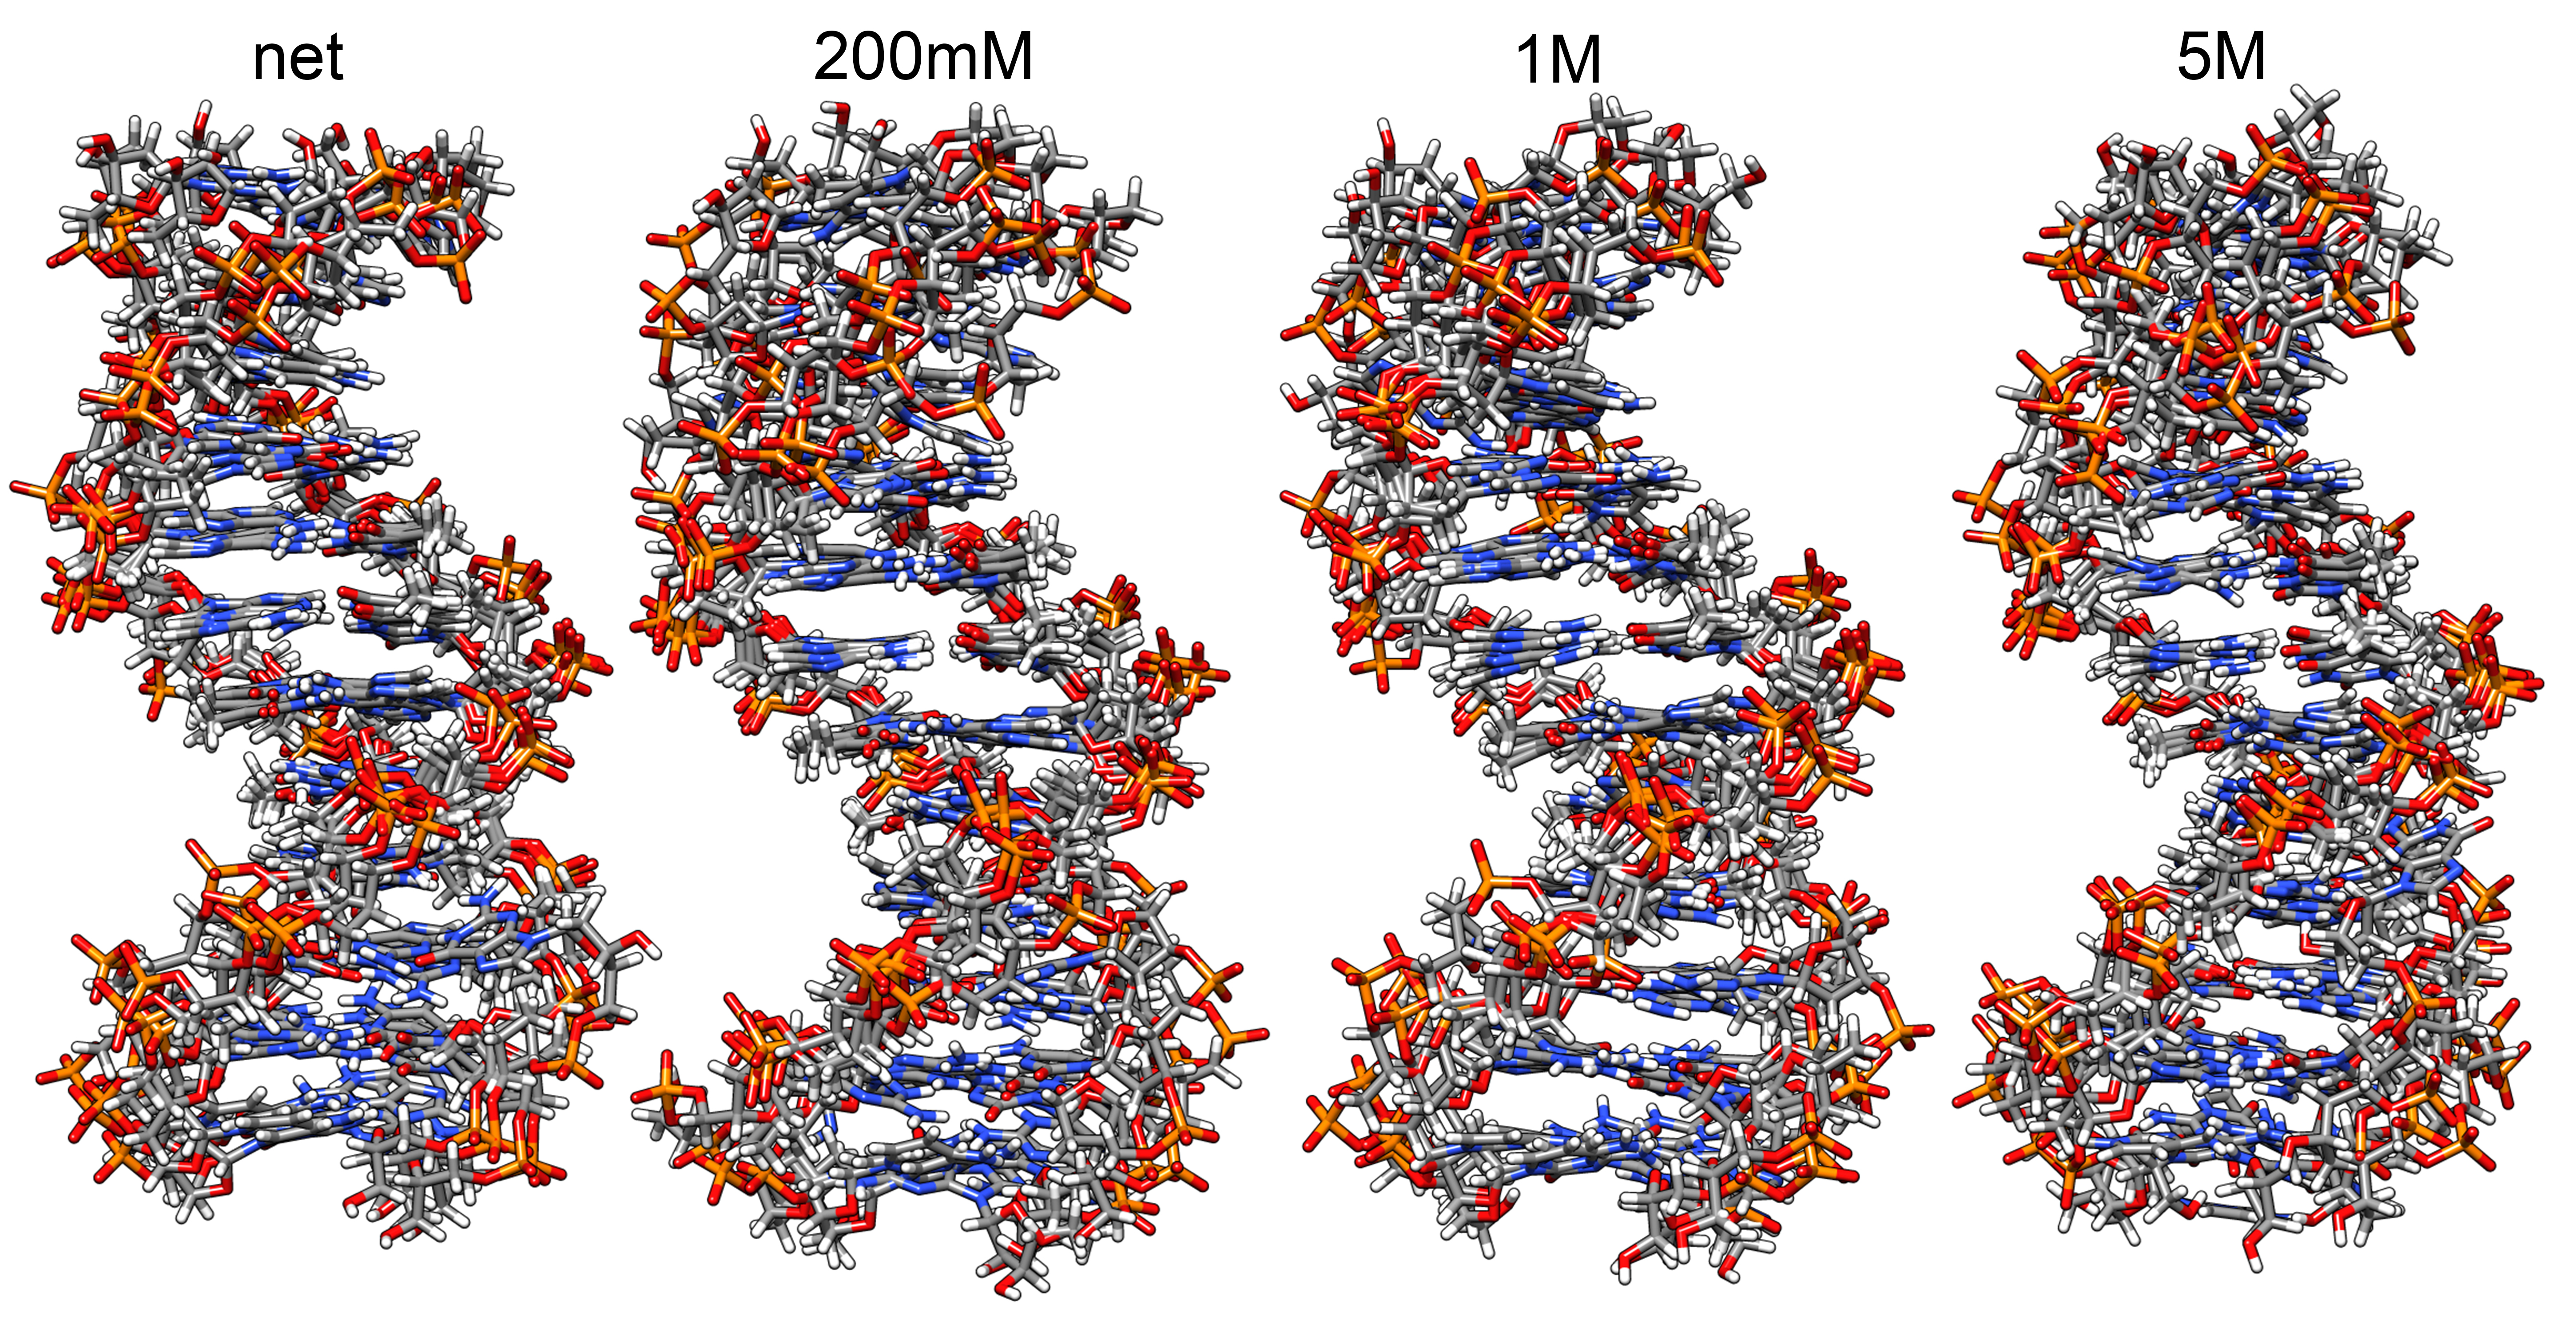
\includegraphics[width=\linewidth]{1us-overlay-all-Cl}
\caption{Overlay of the 1 \SI{}{\micro\second} average structures for LiCl, NaCl, KCl, RbCl and CsCl systems at different salt concentrations.}
\label{1us-overlay-all-Cl}
\end{figure*}



%%%%%%%%%%%%%%%%%%%%%%%%%%%%%%%%%%%%%%%%%%%%%%%%%%%%%%%%%%%%
%%% METHODOLOGY
%%%%%%%%%%%%%%%%%%%%%%%%%%%%%%%%%%%%%%%%%%%%%%%%%%%%%%%%%%%%
\section{Theory and Methods}

The initial model B-DNA structure used for this study was the
Dickerson dodecamer d(CGCGAATTCGCG)$_{2}$, PDB code
1BNA\cite{Drew1981}. A total of 55 simulations were performed starting
from this structure using the various combinations of cations, anions
and concentrations, and each MD simulation was run for at least
\SI{1}{\micro\second}. The parm99\cite{Cheatham3rd1999} force field
with the $\alpha$/$\gamma$ parmbsc0 modifications\cite{Perez2007} were
used with the Joung-Cheatham\cite{Joung2008,Joung2008a} ion parameters
for Li$^{+}$, Na$^{+}$, K$^{+}$, Rb$^{+}$, Cs$^{+}$, Cl$^{-}$,
Br$^{-}$ and I$^{-}$. Ions were added initially to neutralize the
negative charge of the DNA backbone (net neutralizing ions). Then,
additional ions were added to reach a concentration of either
$\sim$0.2M, $\sim$1M or $\sim$5M based on the initial volume of the
constructed periodic cell. To provide further baseline sets of
simulations, single runs were performed using the force fields
ff94\cite{Cornell1995} + parmbsc0, ff98\cite{Cheatham3rd1997} +
parmbsc0 and ff99\cite{Cheatham3rd1999} + parmbsc0 with net
neutralizing NaCl ions. All the systems were solvated with the
TIP3P\cite{Jorgensen1983} water model in a truncated octahedral box
using a 15 Å water shell between the solute and the edge of the
box. To avoid any biases, the initial ion positions were swapped by a
random water molecule using the randomizeions command in CPPTRAJ or
ptraj\cite{Roe2013,Roe2018}.

This starting structure was then used to perform an initial
equilibration phase where the DNA molecule was positionally restrained
using a 25 kcal/mol-Å$^2$ force constant and 500 steps of steepest
descent minimization, switching to 500 steps of conjugate gradient
minimization. Heating was then performed using the same positional
restraints starting at a temperature of 150 K and scaled up to 300 K
using 500 ps of MD simulation using the Langevin\cite{Pastor1988}
thermostat at constant volume. This was followed with a series of
minimization and equilibrium steps slowly decreasing the positional
restraint applied to the DNA from 5 to 0.5 kcal/mol-Å$^2$ using 2 ns
in each step in constant pressure MD simulations. A 2 fs time step was
used with a direct space cut off of 9.0 Å. Trajectory information was
saved every 1 picosecond and the particle mesh Ewald\cite{Darden1993}
method was used to treat long range electrostatic interactions. The
size for the periodic box was set to 69.787 in each direction using a
value of 109.471 for $\alpha,\beta$ and $\gamma$. The PME grid (NFFT1,
NFFT2 and NFFT3) was set to 72 with an Ewald Coefficient of 0.34864. A
total production simulation time of no less than \SI{1}{\micro\second}
was run for every system in the absence of restraints using combined
CPU and GPU technology and the PMEMD module of
AMBER12\cite{Goetz2012}.

In addition to these simulations, due to lack of convergence and
unclear statistical certainty regarding the observed structural
differences from simulations on the \SI{1}{\micro\second} time
scale\cite{Galindo-Murillo2014,Galindo-Murillo2014a}, we extended our
dataset to include trajectories up to \SI{15}{\micro\second} of
sampling time. This second round of data used the same minimization
and equilibration procedure as described and all possible pair
combinations of cations and ions from the set of Li$^{+}$, Na$^{+}$,
K$^{+}$ with Cl$^{-}$ and Br$^{-}$ ions with the same ion model as
studied previously.  The optimum point charge (OPC\cite{Izadi2014})
water model and the OL15\cite{Galindo-Murillo2016} force field were
employed instead. All the MD simulations were performed using either
AMBER12 and AMBER14\cite{Case2005} suite of programs.  Trajectory
analysis was performed using CPPTRAJ version 15.00b available in
AmberTools14\cite{Roe2013,Roe2018}. Average structures of the DNA were
created by a straight coordinate average over all MD trajectory frames
after imaging and RMS fitting to an appropriate reference structure. Clustering analysis was performed using the average linkage clustering algorithm\cite{shao2007} with an epsilon value of 2.0 as
implemented in CPPTRAJ. Only the 10 central base pairs were considered for the clustering analysis.
DNA structural and ion analyses were performed using Curves+, Canal and
Canion\cite{Lavery2014,Lavery2009}.



%%%%%%%%%%%%%%%%%%%%%%%%%%%%%%%%%%%%%%%%%%%%%%%%%%%%%%%%%%%%
%%% RESULTS
%%%%%%%%%%%%%%%%%%%%%%%%%%%%%%%%%%%%%%%%%%%%%%%%%%%%%%%%%%%%
\section{Results and Discussion}

Molecular dynamics simulations were performed to determine if and how
the different salt combinations and concentrations influenced the
structure and dynamics of an experimentally well-studied 12-mer duplex
DNA. Our first observations, based on MD simulations of up to
\SI{1}{\micro\second} (which were representative of the longest
timescale MD simulation studies published investigating the influence
of salt identity and concentration on nucleic acid up to the 2018 time
frame), generated initially inconclusive results. Specifically,
structural differences \textit{were} seen, however the differences in
observed RMSD values of > 1 Å proved to be greater than are expected
for converged DNA helix simulations where RMSD values of < 1 Å are
observed\cite{Galindo-Murillo2014,Galindo-Murillo2014a}.

%%%%%%%%%%%%%%%%
%%   TABLE 1  %%
%%%%%%%%%%%%%%%%
\begin{table}[]
\caption{RMS deviation values (Å) for the net neutralizing simulations and alternate conditions. A \SI{1}{\micro\second} average structure was calculated for each case and used as reference. All
  frames in the trajectory were considered for the RMS calculation.  Inner residue values correspond to the RMSD using residues 3 to 10 and 15 to 22 (i.e. omitting the two terminal base pairs on each end of the helix). The Hawkings, Cramer and Truhlar pairwise generalized Born model was used for the GB calculations\cite{gb1996}.}
\label{1us-rmsd-net}
\begin{tabular}{lllll}
 & \multicolumn{2}{l}{All residues} & \multicolumn{2}{l}{Inner residues} \\
             &               & Std. Dev.          &        & Std. Dev.   \\
No salt      & 2.28          & 0.59               & 1.40   & 0.20        \\
Li           & 2.08          & 0.51               & 1.62   & 0.31        \\
Na           & 1.94          & 0.36               & 1.39   & 0.23        \\
K            & 1.98          & 0.58               & 1.43   & 0.28        \\
Rb           & 1.93          & 0.38               & 1.41   & 0.26        \\
Cs           & 2.02          & 0.38               & 1.41   & 0.27        \\
ff94bsc0     & 3.18          & 0.52               & 1.57   & 0.38        \\
ff98bsc0     & 2.09          & 0.35               & 1.84   & 0.22        \\
ff99bsc0     & 2.18          & 0.46               & 1.46   & 0.31        \\
GB           & 4.19          & 0.71               & 3.46   & 0.75       
\end{tabular}
\end{table}

It is important to mention that achieving this amount of sampling time
during the 2012-2013 years, when these simulations were first performed,
included running MD simulations for $\sim$20 days each on a dedicated M2090
NVIDIA GPU. The following years, new GPU code performance
optimizations\cite{Goetz2012,Salomon-Ferrer2013} and increases in the
performance of the GPU cards coupled with the availability of more
up-to-date AMBER force fields both for nucleic acids and water models,
inspired us to continue our study of ion dependency with a new set of
better converged MD trajectories on the \SI{15}{\micro\second} time
scale. We present both our earlier and the newer results which allows
a direct comparison between converged and non-converged MD
simulations. The results also show the importance and influence of sampling
time and how the results from shorter non-converged simulations can be
misleading.

\subsection{Simulations covering the \SI{1}{\micro\second} timescale.}

Our first dataset consisted of independent simulations of each of the
cations Li$^{+}$, Na$^{+}$, K$^{+}$, Rb$^{+}$ and Cs$^{+}$ paired with
each of the anions Cl$^{-}$, Br$^{-}$ and I$^{-}$. The TIP3P water
model\cite{Jorgensen1983} was used with the Joung-Cheatham
parameters\cite{Joung2008,Joung2008a} in a truncated octahedral
periodic box. These simulations represent our first attempt to study
the influence of different salt concentrations and identities on
duplex DNA and, as mentioned, date back as far as 2012. We present
this dataset as a legacy example that will provide a starting point
for the present work.
 
The RMSD values for the net-neutralizing monovalent salt simulations
are presented in Table \ref{1us-rmsd-net} showing values suggesting
structural differences ranging between 1.93 and 2.08 Å. These values
are reduced by $\sim$0.5 Å when only the central 10 base pairs are
considered indicating that a significant source for the deviation from
the average is the dynamics of the DNA base pairs located at both ends
or termini of the helix, as was been discussed previously in the
literature\cite{Galindo-Murillo2014a,Zgarbova2014}. The no-salt
condition, which is a MD simulation where no net-neutralizing salt is
present, shows a slightly higher deviation of 2.28 Å. On the
\SI{1}{\micro\second} time scale, the DNA helix does not denature as might be
expected, albeit the time scale for this process is not obvious.
The largest RMSD (4.19 Å), a value higher than expected for a good
fidelity simulation of a DNA duplex, was observed in analysis of the
GB implicit solvent simulation. Visual inspection of this implicit
solvent trajectory shows multiple fraying events on both sides of the
DNA chain with a frequent number of backbone transitions to ladder
like structures\cite{Banas2010}, untwisting, and sampling of
non-canonical configurations throughout the simulation.

The MD simulations for each of the salts at the various concentrations
(200mM, 1M and 5M) led to RMS deviations in the range of $\sim$0.8-2.5 Å
(Figure \ref{1us-rms-ALL-inner-avg_ref-bsc0}). The RMSD calculation
was performed with reference to the net-neutralizing (NaCl)
\SI{1}{\micro\second} MD simulation average structure. Overlaying the
population distributions (normalized to 1) in each test
case we detect differences within 1 Å, except for the Cl$^{-}$ case at
1 M, where the difference among the sampled trajectories is $\sim$0.25 Å
(inner residues). Differences in the RMSD histograms in \ref{1us-rms-ALL-inner-avg_ref-bsc0} suggest sampling of different populations of structures or structural differences, however these differences disappear as the structures converge. Analysis performed using the 12 base pairs renders
an increase in the RMS deviation among the simulations due to terminal
base pair fluctuations.  This effect can be observed in the RMS
fluctuation plots (bottom, Figure
\ref{1us-rms-ALL-inner-avg_ref-bsc0}) were we can detect increased
dynamics at both ends of the DNA duplex (within the $\sim$2-3 Å range) and
a small ($\sim$0.25 Å) divergence in dynamics for the central base
pairs. The 200mM NaBr and NaI outliers present are due to long lived
fraying events where the terminal base flips inside the minor
groove (Figure \ref{1us-NaCl_5M-fray-minor-groove}). As already
mentioned, the source of the deviations among simulations is mainly
due to base pair fraying events that occur at both ends of the DNA
chain as observed in the RMS fluctuation measures in Figure
\ref{1us-rms-ALL-inner-avg_ref-bsc0}. To confirm this fact, the
\SI{1}{\micro\second} average structure was compared among different
systems and simulations to detect any noticeable structural deviation
caused by the ions.  An overlay of selected structures is presented in
Figure \ref{1us-overlay-all-Cl} for the LiCl, NaCl, KCl, RbCl and CsCl
at different concentrations. It is evident from the structures that
the central base pairs show less divergence between the selected
system, whereas both ends of the DNA duplex show significant
structural dynamics. Visual inspection also suggests that the
divergence increases as we increase the ion concentration in the
simulation.

%%%%%%%%%%%%%%%%
%%   TABLE 2  %%
%%%%%%%%%%%%%%%%
\begin{table}[]
\caption{RMS deviations of selected systems.  The comparison is using the \SI{1}{\micro\second} average structures from the net neutralizing simulation and measuring the inner residues 4 to 9 and 16 to 21. “net” refers to net-neutralizing monovalent salt.}
\label{1us-rmsd-net-inner}
\begin{tabular}{lllllll}
\multicolumn{7}{l}{Reference structures are the net neutralizing conditions.} \\
         & Concentration    & Li$^{+}$      & Na$^{+}$ & K$^{+}$ & Cs$^{+}$ & Rb$^{+}$      \\
Li       & net              & --      & 1.53    & 1.09    & 1.09    & 1.06    \\
LiCl     & 200 mM           & 1.21    & 1.21    & 1.17    & 0.99    & 0.95    \\
         & 1 M              & 1.25    & 1.20    & 1.03    & 1.18    & 1.00    \\
         & 5 M              & 1.15    & 1.29    & 1.20    & 0.74    & 0.98    \\
LiBr     & 200 mM           & 1.34    & 0.96    & 1.42    & 1.05    & 1.13    \\
         & 1 M              & 1.12    & 1.30    & 0.74    & 1.05    & 0.97    \\
         & 5 M              & 1.40    & 1.36    & 1.22    & 1.18    & 1.10    \\
LiI      & 200 mM           & 1.12    & 1.31    & 0.87    & 1.00    & 0.96    \\
         & 1 M              & 1.54    & 1.19    & 1.57    & 1.45    & 1.34    \\
         & 5 M              & 1.23    & 1.70    & 1.07    & 1.34    & 1.08    \\
Na       & net              & 1.53    & --      & 1.41    & 1.23    & 1.23    \\
NaCl     & 200 mM           & 1.21    & 0.99    & 1.26    & 0.97    & 0.97    \\
         & 1 M              & 1.65    & 0.92    & 1.43    & 1.23    & 1.23    \\
         & 5 M              & 1.58    & 1.04    & 1.33    & 1.21    & 1.21    \\
NaBr     & 200 mM           & 1.15    & 1.48    & 1.33    & 1.21    & 1.21    \\
         & 1 M              & 1.21    & 1.13    & 1.10    & 0.95    & 0.95    \\
         & 5 M              & 1.57    & 1.22    & 1.30    & 1.26    & 1.26    \\
NaI      & 200 mM           & 1.57    & 1.80    & 1.33    & 1.65    & 1.65    \\
         & 1 M              & 1.20    & 1.09    & 1.02    & 0.94    & 0.94    \\
         & 5 M              & 1.50    & 0.87    & 1.40    & 1.16    & 1.16    \\
K        & net              & 1.09    & 1.41    & --      & 1.20    & 0.91    \\
KCl      & 200 mM           & 1.48    & 1.18    & 1.50    & 1.51    & 1.37    \\
         & 1 M              & 1.12    & 1.30    & 0.90    & 1.13    & 0.93    \\
         & 5 M              & 1.55    & 1.17    & 1.13    & 1.54    & 1.21    \\
KBr      & 200 mM           & 1.19    & 1.28    & 0.96    & 1.13    & 0.94    \\
         & 1 M              & 1.41    & 1.28    & 1.14    & 1.36    & 1.12    \\
         & 5 M              & 1.22    & 1.51    & 0.86    & 1.10    & 0.98    \\
KI       & 200 mM           & 1.32    & 0.92    & 1.34    & 1.13    & 1.11    \\
         & 1 M              & 1.22    & 1.27    & 0.80    & 1.30    & 0.96    \\
         & 5 M              & 1.18    & 1.55    & 1.14    & 1.09    & 1.17   
\end{tabular}
\end{table}

%%%%%%%%%%%%%%%%%
%%   Figure 3  %%
%%%%%%%%%%%%%%%%%
\begin{figure}[h]
\centering
\includegraphics[width=95mm]{1us-NaCl_5M-fray-minor-groove}
\caption{Most populated representative structure from the NaCl - 5M simulation showing a fraying event where the free dG nucleobase flips towards the minor groove and forms base-backbone interactions which stabilizes the mis-pair. Hydrogen atoms are hidden for clarity.}
\label{1us-NaCl_5M-fray-minor-groove}
\end{figure}

%%%%%%%%%%%%%%%%%
%%   Figure 4  %%
%%%%%%%%%%%%%%%%%
\begin{figure*}[h!]
\centering
\includegraphics[width=\linewidth]{10us-rms-ALL-inner-avg}
\caption{Left: normalized RMSD populations at three different concentrations, considering only the internal 10 base pairs. Using the net-neutralizing (NaCl) of the Dickerson dodecamer with a total sampling time of \SI{10}{\micro\second}, we computed and extracted an average structure that was used as a reference for the RMSD calculations. Right: root mean square fluctuations per residue. Top to bottom is 200mM, 1M and 5M respectively. For each cation, there are two lines of the same color representing the Cl$^{-}$ and Br$^{-}$ anion values.}
\label{10us-rms-ALL-inner-avg}
\end{figure*}

In order to confirm the central base pair similarity between the
systems presented in Figure \ref{1us-overlay-all-Cl}, we calculated
the RMS deviation among the inner base pairs considering residues 4 to
9 and 16 to 21 that corresponds to the six central base pairs of our
duplex DNA test sequence. We employed the net neutralizing average
structure as a reference and compared to the systems with the cations
Li$^{+}$, Na$^{+}$ and K$^{+}$ using the three simulated
concentrations as our selected dataset (Table
\ref{1us-rmsd-net-inner}). Considering all the calculated values, the
RMSD deviation ranges between $\sim$0.75 and 1.80 Å with no discernable
trend or preference for any combination of salt or concentration. The
molecular graphics in Figure \ref{1us-overlay-all-Cl} and RMS
deviations reported in Table \ref{1us-rmsd-net-inner} may be (and
previously have been) interpreted to suggest structural differences,
however the statistical significance of these differences is uncertain until longer simulations are performed that reach greater structural convergence.

\subsection{Simulations covering the \SI{15}{\micro\second} timescale.}

Our previous \SI{1}{\micro\second} results showed no discernable
difference or trend among the different salt combinations and/or
concentrations, and it was not clear if the observed differences in
structure and RMSD had any statistical significance. From previous
work, we had observed that in longer simulations (beyond
2-5\SI{}{\micro\second}) RMSD differences between independent
simulations were significantly less than 1 Å for the central base
pairs\cite{Galindo-Murillo2014,Galindo-Murillo2014a}. This led us to
increase the sampling time up to \SI{15}{\micro\second} with the same
Dickerson dodecamer and the cations Li$^{+}$, Na$^{+}$ and K$^{+}$
with the anions Cl$^{-}$ and Br$^{-}$, maintaining the three
concentrations so far tested (200 mM, 1 M and 5 M).  These experiments
were performed during the time when the improved OL15 DNA force field
became available\cite{Galindo-Murillo2016,Zgarbova2015}.  We decided
to test this more up-to-date force field and also to include the
optimal point charge (OPC) water model\cite{Izadi2014} that was
demonstrating promising improvements in simulations of
RNA\cite{Bergonzo2015}.


\begin{figure*}[h]
\centering
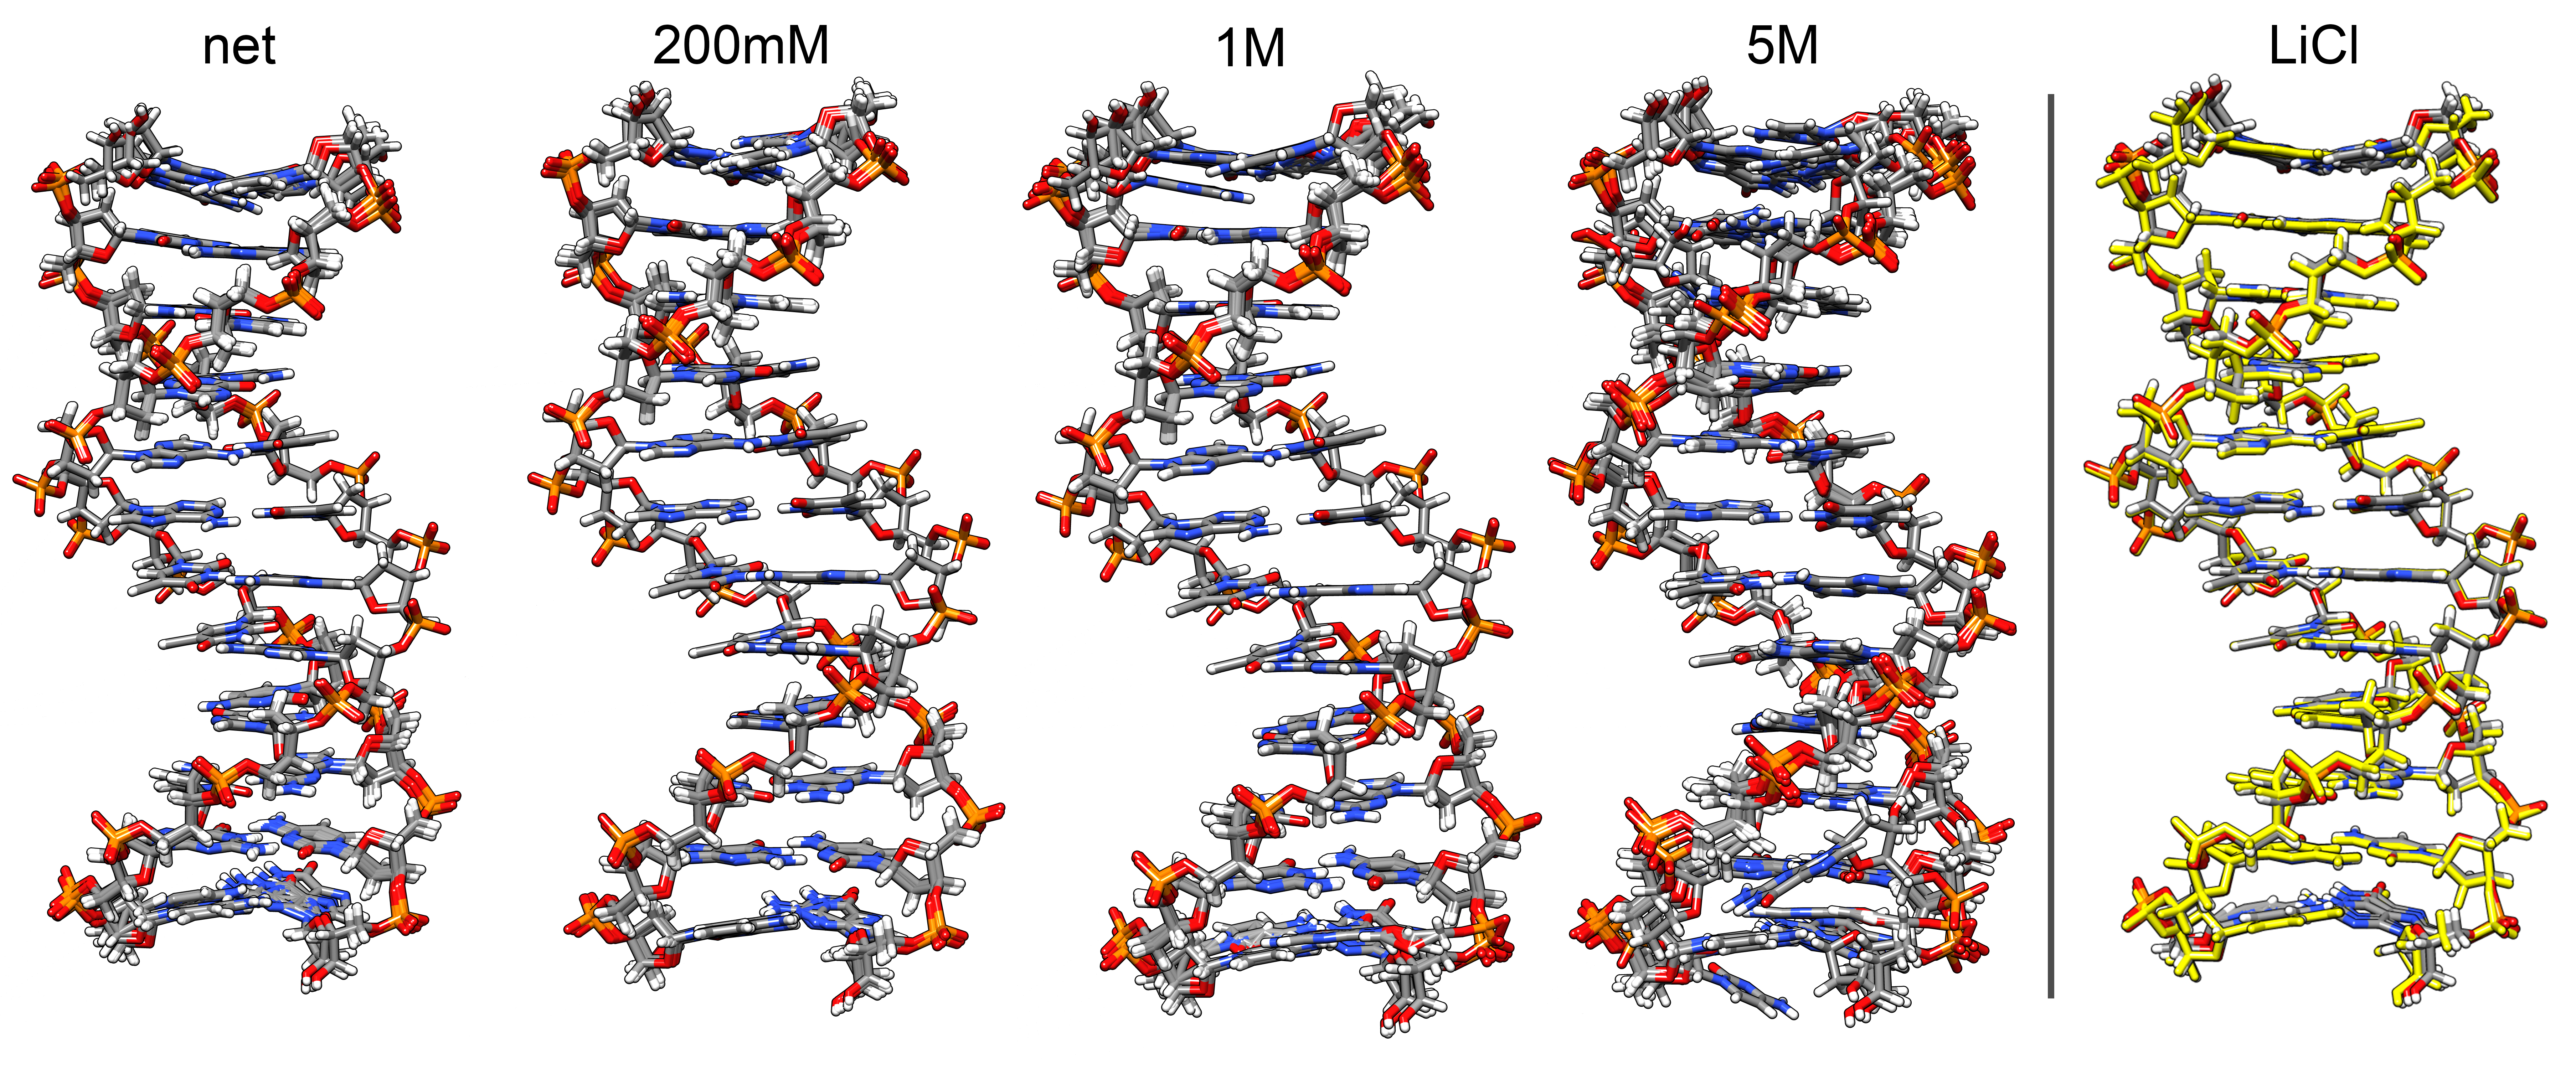
\includegraphics[width=\linewidth]{10us-overlay-all}
\caption{Overlay of the final \SI{10}{\micro\second} average structures for the LiCl, NaCl, KCl, RbCl and CsCl systems at the different salt concentrations. The LiCl structure is an overlay of the \SI{10}{\micro\second} average structure for each salt concentration. Shown in yellow is the 5M concentration average structure.}
\label{10us-overlay-all}
\end{figure*}

The RMS deviation histograms for all the simulated systems present tightly
converged results using the \SI{10}{\micro\second} average structures
as reference (Figure \ref{10us-rms-ALL-inner-avg}). Overall, for the
200 mM and 1 M concentrations, the RMSD populations present
sub-angstrom differences, regardless of cation or anion used. Some
amount of discrepancy is observed for all the 5 M systems, although,
still less than 1 Å. Fluctuations measured using the entire
\SI{15}{\micro\second} trajectory shows the familiar base pair fraying
at both ends of the DNA duplex, with fluctuation values of $\sim$1-1.5 Å
for the inner residues. The simulations using 5 M salt concentration
display the least observed differences among the used cations. To
identify the main source of the structural deviation, we calculated a
\SI{10}{\micro\second} average structure for the Cl$^{-}$ system from
the net, 200 mM, 1 M and 5 M simulations and RMS fit the structures
(Figure \ref{10us-overlay-all}). The similarity of the central base
pairs is between values of $\sim$0.05-0.3 Å whereas the terminal base pairs
present increased fluctuations in the range of $\sim$1-1.5 Å.

\begin{figure*}
\includegraphics[width=\linewidth]{10us-distance-fraying-ALL}
\caption{Normalized population for the distance between the C1’ carbons for first base pair (residues 1 and 24, top) and the 2nd and 3rd base pairs (bottom). Reference value of 10.6 Å is depicted as a gray line in the top plot.}
\label{10us-distance-fraying-ALL}
\end{figure*}

%%%%%%%%%%%%%%%%
%%   TABLE 3  %%
%%%%%%%%%%%%%%%%
\begin{table}[]
\caption{RMS deviations of selected systems.  The comparison is using the \SI{10}{\micro\second} average structures and measuring the inner residues 4 to 9 and 16 to 21 (i.e. neglecting the terminal three base pairs on each end).}
\label{10us-rmsd-inner}
\begin{tabular}{lllll}
\multicolumn{5}{l}{Reference used is the net neutralizing concentration.} \\
             &                & Li$^{+}$      & Na$^{+}$    & K$^{+}$           \\
             & Li net         & --           & 0.24         & 0.11        \\
LiCl         & 200mM          & 0.05         & 0.23         & 0.11        \\
             & 1M             & 0.05         & 0.23         & 0.12        \\
             & 5M             & 0.23         & 0.16         & 0.20        \\
LiBr         & 200mM          & 0.05         & 0.21         & 0.11        \\
             & 1M             & 0.08         & 0.21         & 0.11        \\
             & 5M             & 0.26         & 0.14         & 0.21        \\
             & Na net         & 0.24         & --           & 0.15        \\
NaCl         & 200mM          & 0.18         & 0.09         & 0.11        \\
             & 1M             & 0.09         & 0.18         & 0.10        \\
             & 5M             & 0.26         & 0.34         & 0.27        \\
NaBr         & 200mM          & 0.17         & 0.10         & 0.11        \\
             & 1M             & 0.19         & 0.14         & 0.13        \\
             & 5M             & 0.19         & 0.20         & 0.17        \\
             & K net          & 0.11         & 0.15         & --          \\
KCl          & 200mM          & 0.14         & 0.20         & 0.11        \\
             & 1M             & 0.13         & 0.25         & 0.15        \\
             & 5M             & 0.27         & 0.46         & 0.34        \\
KBr          & 200mM          & 0.07         & 0.19         & 0.06        \\
             & 1M             & 0.09         & 0.27         & 0.15        \\
             & 5M             & 0.54         & 0.49         & 0.50       
\end{tabular}
\end{table}

The magnitude of the difference between selected simulations is
presented in Table \ref{10us-rmsd-inner} where it is remarkable to
notice that the average RMS deviation is only 0.16, 0.21 and 0.16 Å
when using the Li$^{+}$, Na$^{+}$ and K$^{+}$ reference
respectively. The only discernable trend observed is a slight increase
in RMS deviation for the 5 M simulations.

\subsection{Terminal base pair fraying events.}

Fraying events are involved in multiple biological phenomena,
including the recognition for enzymatic catalysis, DNA-enzyme
recogntion, duplex-DNA melting and nuclease
activity\cite{Zgarbova2014}. The dynamic nature of terminal base pair
fraying makes it difficult to study experimentally.  Spin relaxation
measurements on DNA with G:C terminal pairs report motions in the
picosecond to nanosecond time scale\cite{fray09,fray12}.  As a way to
assess these events, we measured the distance between the C1' atoms of
pairing bases. A matched pair is considered to have an average value
of $\sim$10.6 Å between the C1' atoms. The normalized distribution of
distances from our simulations are presented in Figure
\ref{10us-rms-ALL-inner-avg}, where we can see for the base pairs at
the end of the DNA chain (residues 1 and 24) that values other than
10.6 are typically observed.  Visual inspection of the trajectories
suggests that the larger values result from flipped or mis-paired
bases. No clear fraying tendency regarding the specific type of ion is
observed, potentially with the exception of Na$^{+}$ with the
long-lived terminal base pair opening previously discussed. However,
for the 5M salt concentration, terminal base pair fraying events are
increased, generating multiple alternative conformations,
conformations similar to those previously reported in analysis of DNA
duplex MD simulations\cite{Zgarbova2014}.  Our results also suggest
that the DNA is not significantly affected by the type of ion used in
the simulation, but, as mentioned, by the amount present. Our working
hypothesis to explain the effect of the amount of salt with the DNA
structure, and not the type, is that as salt concentration increases,
the time of residence within the grooves increases, which in turn
allow for an increase in shielding between the negatively charged
phosphate groups.

The low RMS deviations obtained from the \SI{10}{\micro\second}
average structures present small, although, significant differences in some
cases (Table \ref{10us-rmsd-inner}). As we increase the concentration,
fraying events become more frequent and RMS deviation increases. For
example, KBr measured using Na$^{+}$ as a reference with RMS values of
0.19, 0.27 and 0.49 Å for 200mM, 1M and 5M respectively. This trend is
consistent among the majority of the studied systems. When comparing
the simulations using the net neutralizing Na$^{+}$ reference, a
slight increase in the RMS deviation is observed, for example, 0.05 Å
LiCl – 200mM with Li$^{+}$ as reference in contrast with the same
system when using Na$^{+}$ as reference (0.21 Å). After visual
inspection of the average structures and trajectories for the Na$^{+}$
net neutralizing simulation used for the calculations, we found
multiple fraying trapped states consistent with the depiction in
Figure \ref{1us-NaCl_5M-fray-minor-groove} with one of the nucleobases
tipping towards the minor groove which causes the slight increase in
RMS deviations when using this frayed structure as reference.

As a measure of convergence within and between the simulations, we
performed a pairwise RMSD combined clustering analysis using the 200mM, 1M and
5M salt concentrations from the NaCl MD simulations. The analysis
algorithm (hierarchical agglomerative) was set to populate 10 clusters
so we could have an even distribution among the different conditions.
The normalized structure population for each cluster during the
sampled time is presented in Appendix Figure \ref{cpop}. We
observe from the plot and the line crossings that cluster populations
have not stabilized or converged on the \SI{1}{\micro\second} time
scale. On the other hand, when the MD simulations on the
\SI{15}{\micro\second} are analyzed, it is clear that the populations
are fairly well converged after $\sim$\SI{1}{\micro\second} and remain
almost unchanged for the remaining of the sampled time.

\subsection{Analysis of the ion distribution.}

In order to study the effect of increased salt on the duplex DNA
structure, we performed several ion distribution analyses on the
\SI{15}{\micro\second} trajectory of LiCl at net neutralizing, 200mM,
1M and 5M salt concentrations. Calculated Li$^{+}$ isodensity surfaces
for each concentration show accumulation of the ions within the
vicinity of the phosphate groups (Figure
\ref{10us-LiCl-ALL_canion-analysis}, top).  As ion concentration is
increased, the density becomes more pronounced and increased ion
populations are clearly evident within both of the grooves.

By means of the canion ion distribution analysis
software\cite{Lavery2014}, we performed a study of the distribution of
Li$^{+}$ ions at different concentrations (Figure
\ref{10us-LiCl-ALL_canion-analysis}). Briefly, \emph{D} represent the
distance along the helical axis, \emph{A} is an angle that tracks the
helical twist and \emph{R} is the distance from the helical axis towards the solvent. In the \emph{DA} plot, we include two vertical white lines located at 33$\deg$ and 147$\deg$ that delimit the
minor groove region. The net neutralizing concentration shows an accumulation of
ions within the minor groove with highest molarity values close to the central
base pairs and little to no presence inside the major groove. As we
increase the concentration, we observe a strong increase in molarity of ions within the major groove localized mainly within the phosphate groups as observed in the 3D grid density histogram. The
presence of ions within the major groove at 5M is confirmed with the aid of the \emph{RA} and \emph{DR} plots. The white circle in the \emph{RA} plot located at a distance of 10.2 Å from the helical
axis delimits the outer circumference of the DNA duplex and indicates the distance of the C1' carbon atoms. The white radial vectors indicate the groove limits and the center of the major groove
(vertical vector). Similarly, for the \emph{DR} plots, the white line at 10.2 Å
delimits the C1' carbons. This analysis helps
explain why some degree of modest structural difference is observed
mostly only at the 5M salt concentration.

\begin{figure*}[]
\centering
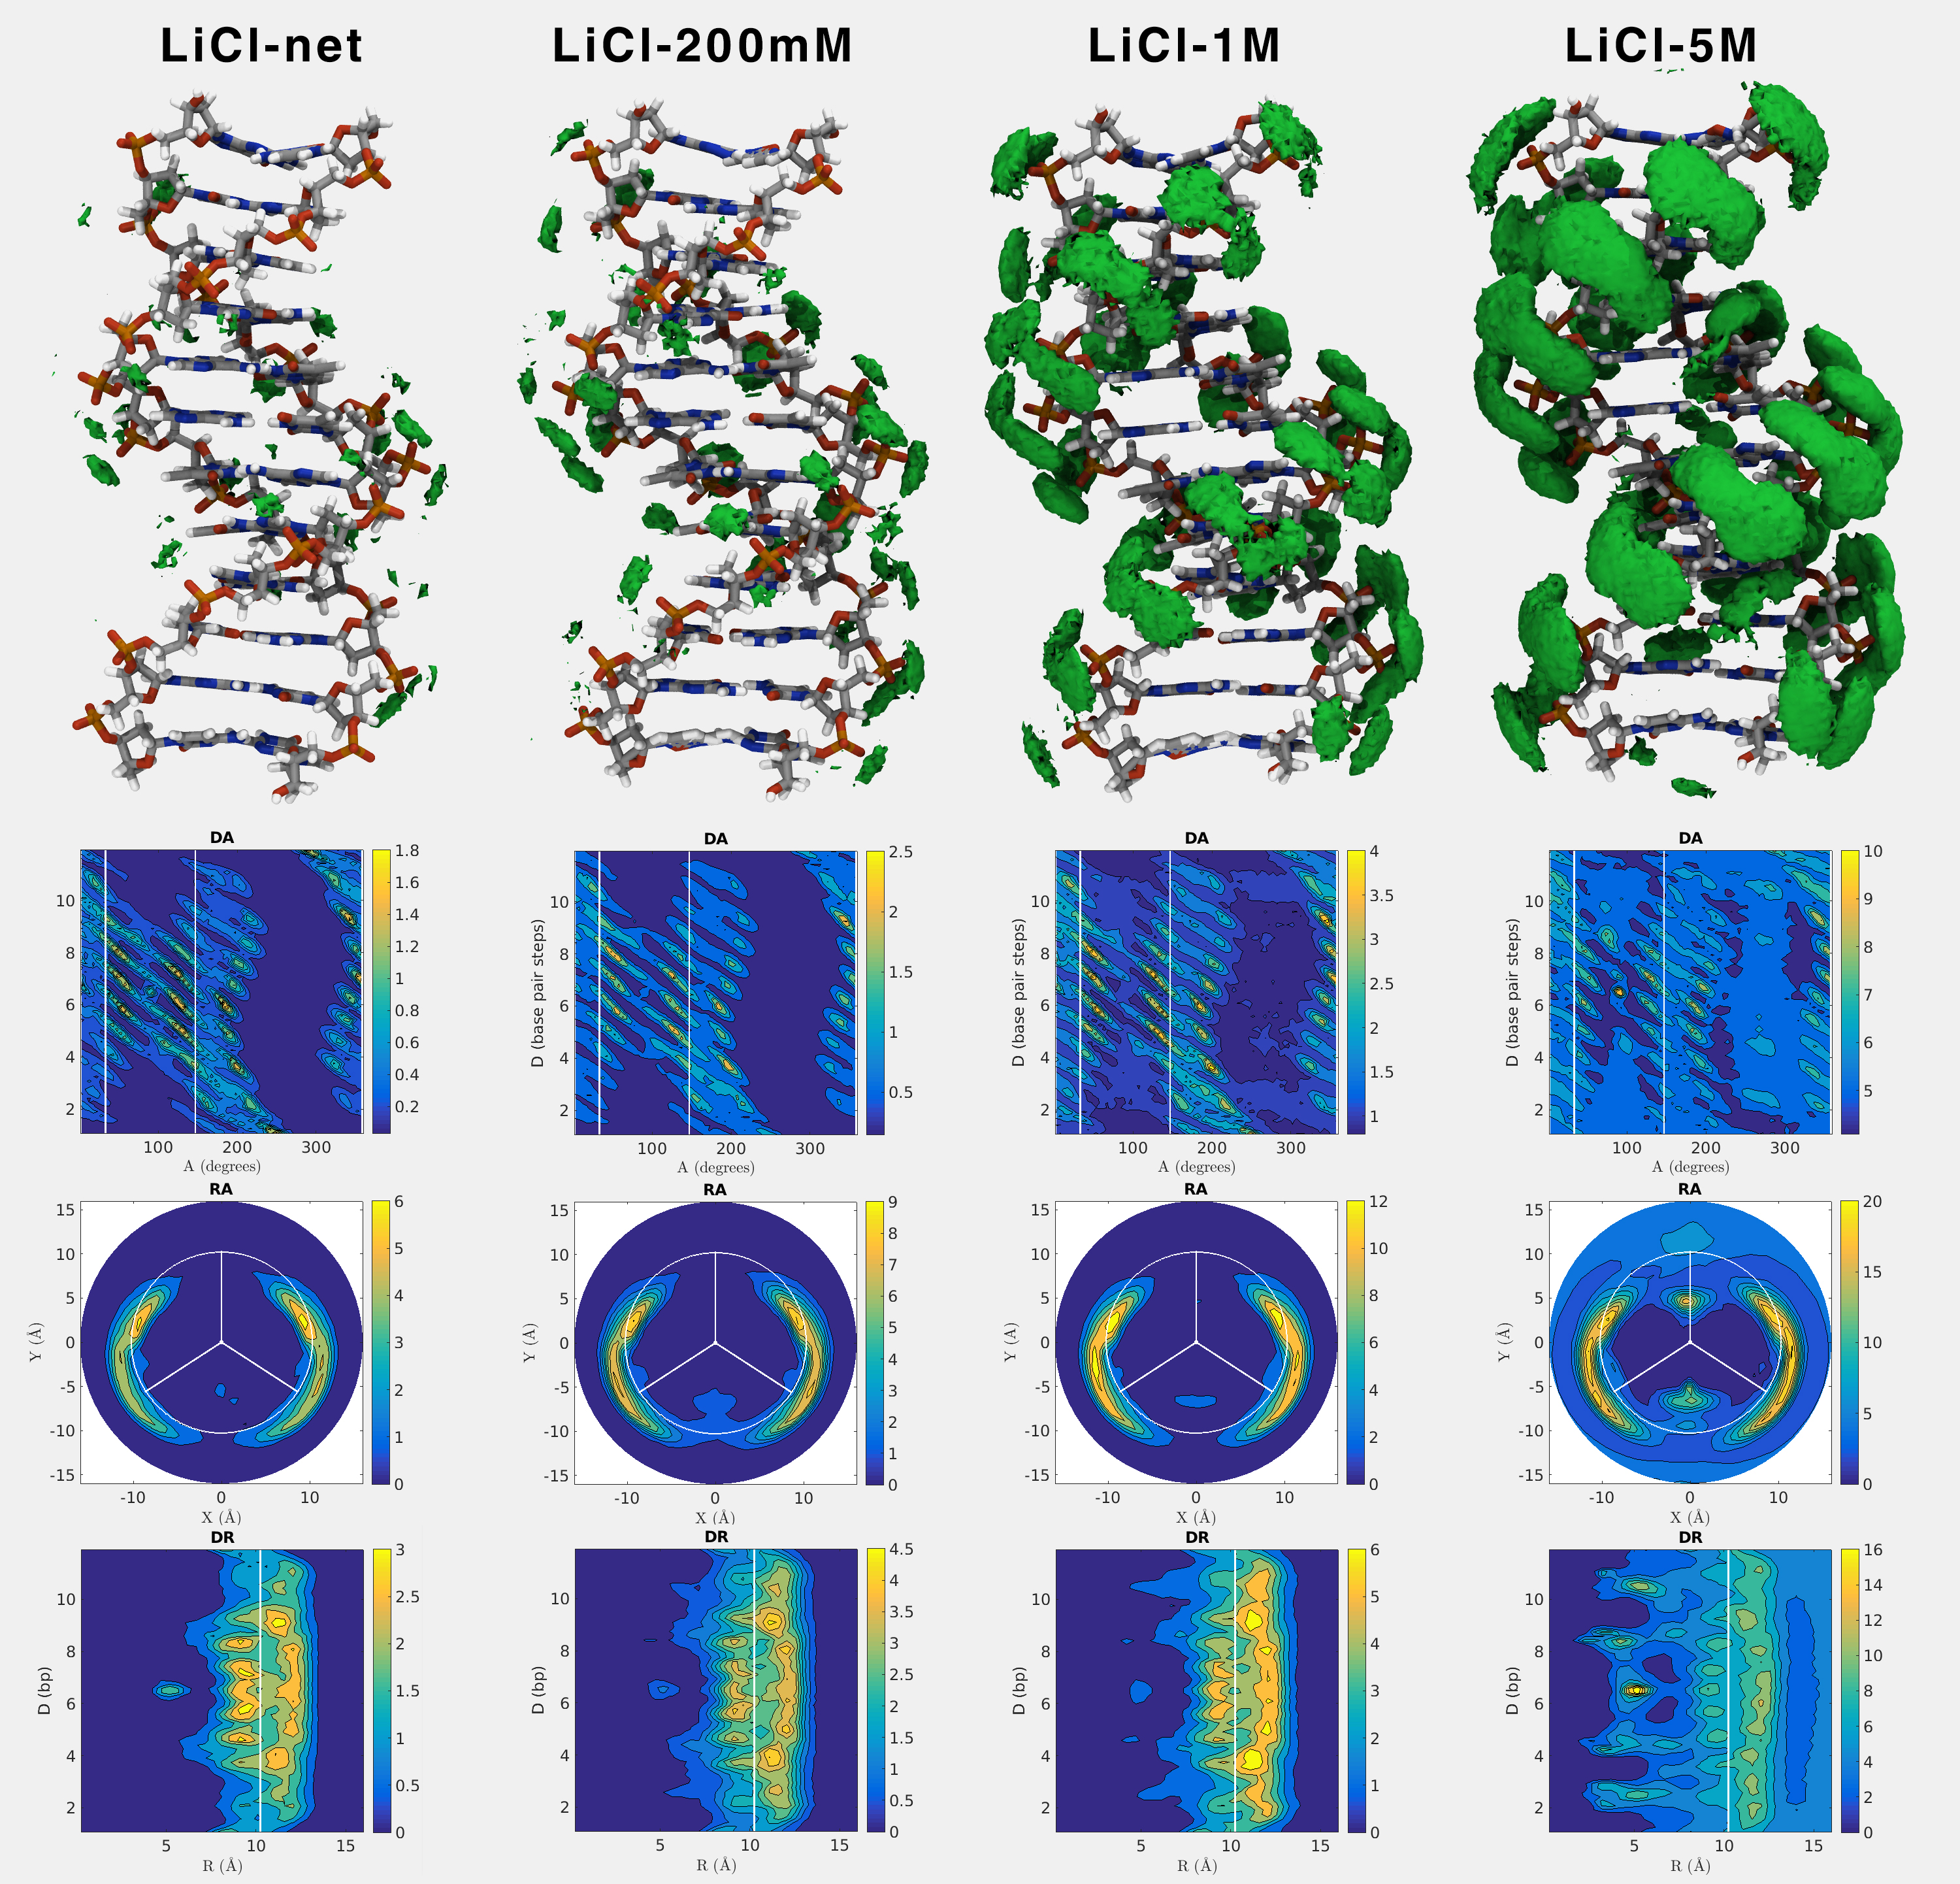
\includegraphics[width=\textwidth,height=18cm]{10us-LiCl-ALL_canion-analysis}
\caption{Top: ion density of Li$^{+}$ (green isosurface value of 0.54). Bottom: 2D ion distributions. The blue to yellow color indicate increasing values of molarity. Notice the difference in molarity
  scales across the net, 200mM, 1M and 5M concentrations. Using the same molarity scale across salt
  concentrations was not possible due to the fact that the scale that rendered a good image for the net/200mM system was completly saturated for the 5M and the scale that showed a balanced image for
  the 5M system would not allow to see any information for the net/200mM system. Allowing the molarity scale to adjust to its optimal value shows more detail in the analysis. The white lines in the \emph{DA}
  plots represent th eminor groove limits as defined by the C1' carbon positions, as with the \emph{DR} plot. The white circle in the \emph{RA} plots represent the radial vector limit for the C1'
  carbons; radial sampling limited to 15 Å. Refer to \cite{Lavery2014} for more information. Analysis calculated using the entire \SI{15}{\micro\second} trajectory.}
\label{10us-LiCl-ALL_canion-analysis}
\end{figure*}

\subsection{Structural analysis.}

To further study the subtle structural influences of the different
salt concentrations on the duplex DNA, noting that helicoidal
parameters are extremely sensitive measures of small differences in
structure, we calculated the helicoidal parameters using the
\SI{10}{\micro\second} average structure for each simulation condition
(Appendix table). There is a reduction on the major groove width as
salt concentration is increased. This reduction is independent of the
type of salt and is observed consistently among the six systems. A
similar reduction in width is observed for the minor groove except for
the systems with the Li$^{+}$ cation where the width value remained
similar for the lower salt concentrations and increased slightly in
the 5M salt simulations. Lower twist values are also observed for the
5M simulations in comparison with the rest of the concentrations
(except for the KCl system). Similar decrease of rise distance between
base pairs is observed as we increase ion concentration. The unwinding
of the DNA in the 5M salt simulations couples with the reduction of
the groove widths, with the exception of slight minor groove width
increase in the Li$^{+}$ simulations which likely is due to the change
in bending which is not observed in the Na$^{+}$ and K$^{+}$ 5M salt
simulations.


%%%%%%%%%%%%%%%%%%%%%%%%%%%%%%%%%%%%%%%%%%%%%%%%%%%%%%%%%%%%
%%% CONCLUSIONS
%%%%%%%%%%%%%%%%%%%%%%%%%%%%%%%%%%%%%%%%%%%%%%%%%%%%%%%%%%%%
\section{Conclusions}

The results presented highlight some of our recent experiences
($\sim$2012-2019) assessing and validating the capabilities of AMBER force
fields parmbsc0 and OL15 to detect and be affected by different salt
types and salt concentrations using the Joung—Cheatham ion
parameters. Our observations suggest:
\begin{itemize}

\item Simulations of $\sim$\SI{1}{\micro\second} or less for a 12- to
  18-mer duplex DNA are definately not converged. MD simulations
  should likely be at least in the range of $\sim$5-10
  \SI{}{\micro\second} time range to be comparable and to assess
  subtle structural differences. As sampling time increases, the
  structural populations of different local-minima approach
  convergence.  With more simulation time, the generated structures
  start to populate a consistent set of representative structures with
  consistent cluster populations for those structures. As the
  simulation time increases, the resulting average structure converges
  to a single representative structure.

\item Regardless of the type of cation or anion used, with these
  additive force fields, the DNA is not significantly affected as
  measured by RMS deviations over averaged structures.

\item As we increase salt concentration, increased fluctuations and
  fraying effects at both ends of the DNA chain increase.

\item Decrease in major groove width, minor groove width (with the
  exception of Li$^{+}$ where the minor groove width increases and
  bending decreases), twist angle and inter base pairs rise as a
  function of increased ion concentration is observed for the 10
  central base pairs.

\item With these force fields, DNA helices in the absence of salt do
  not denature in simulations on the \SI{1}{\micro\second} time scale.

\end{itemize}

We take this opportunity of reporting our results in this version of
the “Lessons Learned” category of the Living Journal of Computational
Molecular Science to share with any research group that is interested
in studying the effects of high salt concentration in DNA using AMBER
in the hopes that they will find our experience useful. The next step
for updating our work will be incorporating the parmbsc1 variation of
the AMBER DNA force field, exploring different water models,
performing longer no-salt DNA simulations, and explorations of new
nucleic acid polarizable force fields\cite{Li2017} in the hope of
learning the source for, or to verify the, lack of sensitivity of DNA
simulations to strong ionic environment.

Pre-processed trajectories and topology files are available for
download at: http://www.amber.utah.edu/DNA-dynamics/livecoms-salt/



\section{Author Contributions}
%%%%%%%%%%%%%%%%
% This section mustt describe the actual contributions of
% author. Since this is an electronic-only journal, there is
% no length limit when you describe the authors' contributions,
% so we recommend describing what they actually did rather than
% simply categorizing them in a small number of
% predefined roles as might be done in other journals.
%
% See the policies ``Policies on Authorship'' section of https://livecoms.github.io
% for more information on deciding on authorship and author order.
%%%%%%%%%%%%%%%%

RG-M and TEC3 contributed equally in this article. For a more detailed description of author contributions, see the GitHub issue tracking and changelog at \githubrepository.

\section{Funding Information}
%%%%%%%
% Authors should acknowledge funding sources here. Reference specific grants.
%%%%%%%
TEC3 acknowledges the support of NIH grant GM081411.

\bibliography{refs}

%%%%%%%%%%%%%%%%%%%%%%%%%%%%%%%%%%%%%%%%%%%%%%%%%%%%%%%%%%%%
%%% APPENDICES
%%%%%%%%%%%%%%%%%%%%%%%%%%%%%%%%%%%%%%%%%%%%%%%%%%%%%%%%%%%%

\appendix


\clearpage

\begin{landscape}


  \begin{table}[]
\caption{Selected helicoidal parameters calculated from a 10 $\mu$s average structure for each system. Standard deviation calculated from the 10 $\mu$s trajectory data. NMR reference data obtained
  from the PDB code 1NAJ. All the data is calculated using the central base-pairs only (3-10 and 15-22)}
\centering
\resizebox{\textwidth}{!}{%
\begin{tabular}{llllllllllllllllllllllllllllll}
  &  &  Major & Std. Dev. & Minor & Std. Dev.& H-rise & Std. Dev.& H-twist & Std. Dev. & Stretch & Std. Dev.& Stagger & Std. Dev.& Buckle & Std. Dev.& Propeller & Std. Dev.& Slide & Std. Dev.& Rise &
  Std. Dev.& Roll &Std. Dev. & Twist & Std. Dev.& Inclination & Std. Dev. & Bend &  \\
  NMR ref & & 11.52 & & 4.18& & 3.20& & 36.2& & -0.30& & -0.07& & -0.0& & -18.1& & -0.15& & 3.20& & 2.9& & 36.0& & 3.7& & 1.6 \\
  LiCl & net & 11.82 & 1.38 & 3.78 & 1.33 & 3.33 & 0.30 & 36.0 & 5.5 & -0.03 & 0.11 & 0.08 & 0.38 & -0.0 & 10.5 & -12.5 & 10.0 & -0.06 & 0.66 & 3.32 & 0.28 & 1.6 & 6.3 & 35.9 & 5.6 & 1.8 & 5.9 & 1.0 &
  0.9 \\
 & 200mM & 11.81 & 1.38 & 3.78 & 1.35 & 3.33 & 0.30 & 35.9 & 5.6 & -0.04 & 0.11 & 0.07 & 0.38 & -0.0 & 10.5 & -12.5 & 9.9 & -0.03 & 0.67 & 3.32 & 0.28 & 1.8 & 6.3 & 35.8 & 5.7 & 2.0 & 5.9 & 1.0
  & 0.9 \\
 & 1M & 11.71 & 1.37 & 3.76 & 1.33 & 3.33 & 0.30 & 36.1 & 5.6 & -0.03 & 0.11 & 0.08 & 0.38 & 0.1 & 10.5 & -12.6 & 10.0 & -0.04 & 0.66 & 3.32 & 0.28 & 1.8 & 6.2 & 36.0 & 5.6 & 2.0 & 5.8 & 0.9 & 0.9 \\
 & 5M & 11.43 & 1.37 & 3.88 & 1.33 & 3.31 & 0.30 & 35.7 & 5.6 & -0.03 & 0.11 & 0.06 & 0.38 & -0.4 & 10.5 & -12.6 & 10.0 & -0.02 & 0.6 & 3.31 & 0.28 & 2.4 & 6.2 & 35.6 & 5.6 & 3.2 & 5.8 & 0.6 & 0.9  \\
  LiBr & net & 11.84 & 1.38 & 3.78 & 1.35 & 3.34 & 0.30 & 36.1 & 5.6 & -0.03 & 0.11 & 0.08 & 0.38 & -0.1 & 10.5 & -12.5 & 9.9 & -0.06 & 0.67 & 3.32 & 0.28 & 1.6 & 6.3 & 36.0 & 5.6 & 1.7 & 5.9 & 0.9 & 0.9 \\
 & 200mM & 11.75 & 1.37 & 3.76 & 1.35 & 3.33 & 0.30 & 35.9 & 5.6 & -0.03 & 0.11 & 0.07 & 0.38 & 0.0 & 10.6 & -12.5 & 10.1 & -0.04 & 0.67 & 3.32 & 0.29 & 1.8 & 6.3 & 35.9 & 5.7 & 2.1 & 5.9 & 0.9
  & 0.9 \\
 & 1M & 11.75 & 1.37 & 3.81 & 1.36 & 3.33 & 0.30 & 35.8 & 5.6 & -0.03 & 0.11 & 0.06 & 0.38 & -0.1 & 10.5 & -12.5 & 9.9 & -0.02 & 0.68 & 3.31 & 0.29 & 1.9 & 6.3 & 35.7 & 5.7 & 2.3 & 5.9 & 1.0 &
  0.9 \\
 & 5M & 11.53 & 1.36 & 3.96 & 1.36 & 3.31 & 0.30 & 35.5 & 5.6 & -0.03 & 0.11 & 0.05 & 0.38 & -0.1 & 10.5 & -12.5 & 9.8 & -0.01 & 0.68 & 3.30 & 0.29 & 2.4 & 6.3 & 35.4 & 5.7 & 3.3 & 5.9 & 0.6 & 0.9 \\
  NaCl & net & 11.88 & 1.40 & 4.10 & 1.37 & 3.33 & 0.30 & 35.6 & 5.8 & -0.03 & 0.11 & 0.05 & 0.38 & 0.2 & 10.6 & -11.8 & 10.0 & -0.10 & 0.67 & 3.32 & 0.29 & 2.3 & 6.2 & 35.5 & 5.8 & 3.0 & 5.8 & 0.9 &
  0.9 \\
 & 200mM & 11.82 & 1.39 & 4.04 & 1.37 & 3.33 & 0.30 & 35.8 & 5.7 & -0.04 & 0.11 & 0.06 & 0.38 & 0.0 & 10.6 & -12.3 & 9.9 & -0.08 & 0.67 & 3.32 & 0.29 & 2.3 & 6.2 & 35.7 & 5.8 & 2.8 & 5.8 & 0.9 &
  0.9 \\
 & 1M & 11.73 & 1.38 & 3.91 & 1.35 & 3.33 & 0.29 & 36.0 & 5.7 & -0.03 & 0.11 & 0.08 & 0.38 & 0.0 & 10.6 & -12.7 & 9.9 & -0.06 & 0.66 & 3.32 & 0.28 & 2.0 & 6.2 & 35.9 & 5.7 & 2.2 & 5.9 & 0.9 &
  0.9 \\
 & 5M & 11.71 & 1.37 & 3.52 & 1.34 & 3.29 & 0.30 & 35.3 & 5.7 & -0.03 & 0.11 & 0.11 & 0.38 & 0.6 & 10.6 & -12.7 & 9.0 & -0.01 & 0.66 & 3.28 & 0.28 & 1.5 & 6.2 & 35.2 & 5.7 & 1.5 & 5.9 & 1.1 & 0.9 \\
  NaBr & net & 11.92 & 1.40 & 4.10 & 1.38 & 3.33 & 0.30 & 35.7 & 5.7 & -0.04 & 0.12 & 0.06 & 0.38 & -0.1 & 10.6 & -12.1 & 9.8 & -0.10 & 0.67 & 3.33 & 0.29 & 2.3 & 6.2 & 35.6 & 5.8 & 2.9 & 5.8 & 0.9 &
  0.9 \\
 & 200mM & 11.82 & 1.38 & 4.05 & 1.37 & 3.33 & 0.30 & 35.8 & 5.7 & -0.03 & 0.11 & 0.07 & 0.38 & -0.1 & 10.6 & -12.3 & 9.8 & -0.09 & 0.67 & 3.32 & 0.29 & 2.2 & 6.2 & 35.7 & 5.7 & 2.7 & 5.8 & 0.9
  & 0.9 \\
 & 1M & 11.68 & 1.39 & 3.91 & 1.38 & 3.31 & 0.30 & 35.5 & 5.9 & -0.03 & 0.12 & 0.05 & 0.38 & 0.3 & 10.7 & -12.0 & 10.2 & -0.04 & 0.67 & 3.31 & 0.29 & 2.0 & 6.2 & 35.4 & 6.0 & 2.7 & 5.9 & 0.9 &
  0.9 \\
 & 5M & 11.91 & 1.39 & 3.80 & 1.38 & 3.30 & 0.30 & 35.4 & 5.9 & -0.04 & 0.12 & 0.10 & 0.38 & -0.1 & 10.7& -14.0 & 10.2 & -0.05 & 0.67 & 3.29 & 0.29 & 2.3 & 6.2 & 35.2 & 6.0 & 2.7 & 5.9 & 1.0 & 0.9  \\
 KCl & net & 11.92 & 1.39 & 3.91 & 1.31 & 3.33 & 0.30 & 35.8 & 5.8 & -0.03 & 0.11 & 0.07 & 0.38 & 0.1 & 10.6 & -12.1 & 10.2 & -0.11 & 0.67 & 3.32 & 0.29 & 2.0 & 6.2 & 35.6 & 5.9 & 2.3 & 5.8 & 1.0 &
  0.9 \\
 & 200mM & 11.80 & 1.39 & 3.88 & 1.32 & 3.32 & 0.30 & 35.6 & 5.7 & -0.03 & 0.12 & 0.07 & 0.38 & -0.2 & 10.6 & -12.0 & 10.1 & -0.08 & 0.67 & 3.31 & 0.29 & 2.0 & 6.2 & 35.5 & 5.9 & 2.3 & 5.9 & 1.0
  & 0.9 \\
 & 1M & 11.67 & 1.36 & 3.75 & 1.36 & 3.32 & 0.31 & 35.6 & 5.9 & -0.03 & 0.11 & 0.09 & 0.38 & -0.1 & 10.8 & -12.5 & 10.0 & -0.04 & 0.68 & 3.31 & 0.30 & 1.9 & 6.3 & 35.4 & 6.1 & 2.2 & 6.0 & 1.1 &
  0.9 \\
 & 5M & 11.48 & 1.36 & 3.40 & 1.36 & 3.30 & 0.31 & 35.7 & 5.9 & -0.04 & 0.12 & 0.13 & 0.38 & -0.1 & 10.1 & -13.0 & 10.0 & -0.01 & 0.68 & 3.29 & 0.30 & 1.3 & 6.3 & 35.6 & 6.1 & 0.9 & 6.0 & 1.2 &  0.9  \\
  KBr & net & 11.95 & 1.40 & 3.93 & 1.33 & 3.33 & 0.30 & 35.7 & 5.7 & -0.04 & 0.11 & 0.07 & 0.38 & 0.1 & 10.5 & -12.1 & 9.9 & -0.10 & 0.68 & 3.32 & 0.29 & 2.1 & 6.3 & 35.6 & 5.8 & 2.4 & 5.8 & 1.1 &
  0.9 \\
  & 200mM & 11.85 & 1.38 & 3.87 & 1.31 & 3.33 & 0.30 & 35.9 & 5.6 & -0.04 & 0.11 & 0.08 & 0.38 & 0.0 & 10.5 & -12.3 & 9.9 & -0.09 & 0.67 & 3.31 & 0.29 & 1.9 & 6.2 & 35.8 & 5.7 & 2.0 & 5.8 & 1.0 &
  0.9 \\
  & 1M & 11.70 & 1.37 & 3.73 & 1.33 & 3.33 & 0.31 & 35.8 & 5.7 & -0.03 & 0.11 & 0.09 & 0.38 & -0.1 & 10.7 & -12.5 & 10.0 & -0.04 & 0.67 & 3.31 & 0.29 & 1.7 & 6.3 & 35.7 & 5.8 & 1.8 & 5.9 & 1.0 &
  0.9 \\
  & 5M & 11.40 & 1.37 & 3.72 & 1.33 & 3.27 & 0.31 & 34.3 & 5.7 & -0.02 & 0.11 & 0.09 & 0.38 & -0.6 & 10.7 & -13.0 & 10.0 & -0.11 & 0.67 & 3.27 & 0.29 & 2.4 & 6.3 & 34.2 & 5.8 & 3.6 & 5.9 & 1.1 & 0.9  \\
\end{tabular}%
                  }
                  \end{table}

\end{landscape}

\begin{figure*}[h]
\centering
\includegraphics[width=\linewidth]{cpop-NaCl-all}
\caption{Normalized cluster population analysis over time for the \SI{1}{\micro\second} and \SI{15}{\micro\second} simulations. Clustering was performed using the hierarchical agglomerative (bottom-up) approach focusing on the inner 8 residues (3-10 and 15-22). Each line represent one of the 10 calculated clusters for each simulation.} 
\label{cpop}
\end{figure*}



\end{document}
